\chapter{Project Development}

\section{Datasets}
There are several datasets on the internet, but none of them have the amount of sheer volume and actually useful data that is required for this task. The closest available was used, however, and it brought relatively acceptable levels of accuracy \citep{rf7}.
This dataset, paired with NLTK processing, stopwords and truncating words and verbs commonly used in the English language, was able to pinpoint if the user had a positive, neutral or a negative feeling in their input about 40\% of the time, approximately.
This is not really a good number for such a small amount of labels, but it's an improvement nonetheless. Previous versions with different approaches, combination of layers and datasets had less than 20\% of accuracy.
\pagebreak

\subsection{Pre-filtering}
Since the dataset that was chosen was imported straight from Twitter with little to no filtering, some cleanup had to be done to ensure peak performance.
The first problem was the punctuation marks, which were easy to filter out. The issues came after this with the so-called stopwords, which are words that don't really contribute to the overall meaning of the text. Luckily, NLTK\footnote{Natural Language Toolkit, tool used specifically for these case scenarios. \url{https://www.nltk.org/}} has its own repository of these words, so it was implemented. There was also an issue where verbs in different tenses were evaluated very differently, so a  stemmer was implemented, which truncated words to its most basic features (aptly named stems) and prevented the loss to keep rising that much between epochs.
\pagebreak
\begin{figure}[!h]
	\centering
	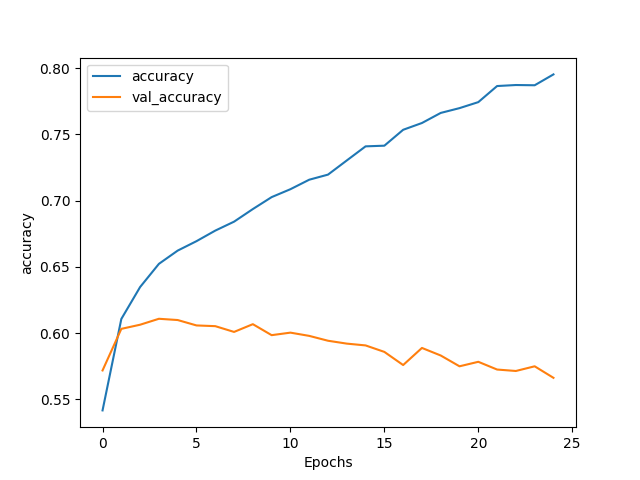
\includegraphics[scale=0.6]{Accuracy 2020-05_nofilter}
	\caption{Accuracy Graph of the Algorithm Training on May 2020, with no NLTK stemming}
	\label{fig:accuracy2020_nofilter}
	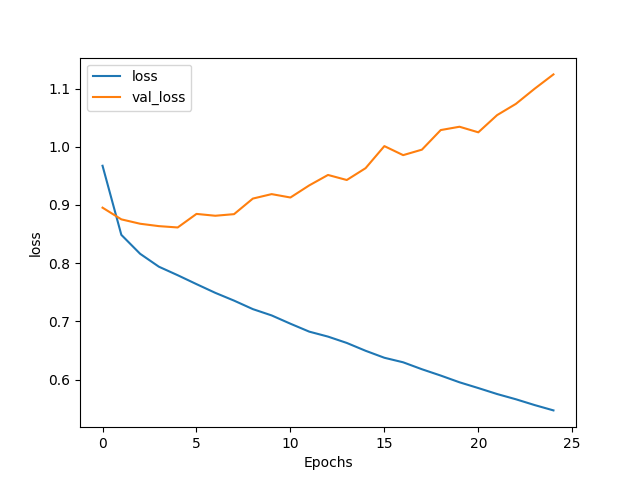
\includegraphics[scale=0.6]{Loss 2021-05}
	\caption{Loss Graph of the Algorithm Training on May 2020, with no NLTK stemming}
	\label{fig:loss2020_nofilter}
\end{figure}

\subsection{Filtering}
The dataset itself has several different sentiment labels to analyze, the ones being considered in the scope of this paper are:
\begin{itemize}
	\item Sadness
	\item Neutral
	\item Happiness
	\item Fun
	\item Worry
	\item Boredom
\end{itemize}
But since they're not evenly distributed, leaving them as-is led to very inaccurate results, so a generalistic approach was opted for, classifying the end results in "Good", "Neutral" and "Bad" depending on the overall wellness of the user.
This final filter works only with the training data, and works as follows:
\begin{itemize}
	\item Sadness and Worry go in the "Bad" category.
	\item Neutral and Boredom go in the "Neutral" category.
	\item Happiness and Fun go in the "Good" category
\end{itemize}
Using a more complicated classification process would take an even amount of data in every category. Which, at the time of writing, there isn't a dataset readily available.

\section{Algorithm Used}
A bidirectional LSTM algorithm was used with a softmax activation end layer. After much, much testing \textit{rmsprop} was chosen as the optimizer because of its slightly better results overall.
The internal lexicon is limited to 5000 items, and the maximum length of any given phrase after filtering is 30 characters.
The training consists in 25 epochs on 75\% of the dataset on a random arbitrary order, using the remaining 25\% for validation instead.
\begin{figure}[!h]
	\centering
	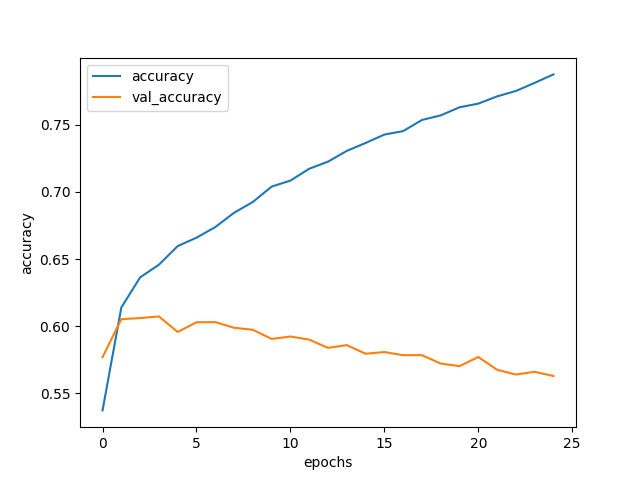
\includegraphics[scale=0.6]{Accuracy 2021-05}
	\caption{Accuracy Graph of the Algorithm Training on May 2021}
	\label{fig:accuracy2021}
	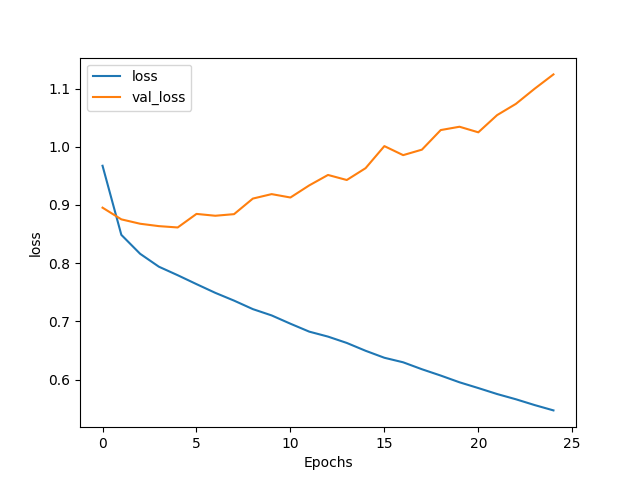
\includegraphics[scale=0.6]{Loss 2021-05}
	\caption{Loss Graph of the Algorithm Training on May 2021}
	\label{fig:loss2021}
\end{figure}
\begin{figure}[!h]
	\centering
	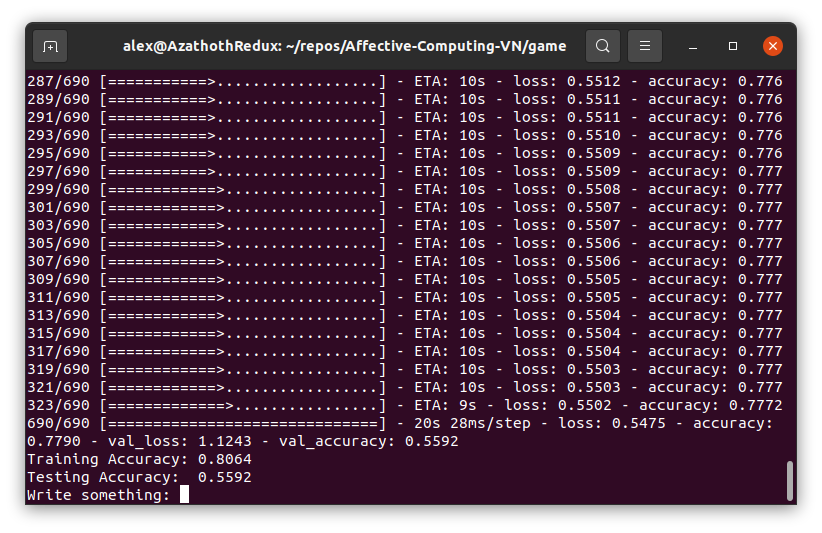
\includegraphics[scale=0.4]{Test 2021-05}
	\caption{Debugging of the Trained Model}
	\label{fig:test}
\end{figure}
\pagebreak

\section{Interface}
Originally, \textit{Ren'py}\footnote{An open-source Python framework focused mostly in the development of visual novels and other videogame formats. \url{https://www.renpy.org/}} was the chosen framework for this project's interface to work with, but -- unfortunately for the proposed usage -- it only works with Python 2.7, which makes it incompatible with TensorFlow 2.0. Making a bridge between Python 2 and 3 would inevitably generate more issues that would take more time to solve, so it was scrapped in favor of the \textit{pygame} library.
\pagebreak

\begin{figure}[!h]
	\centering
	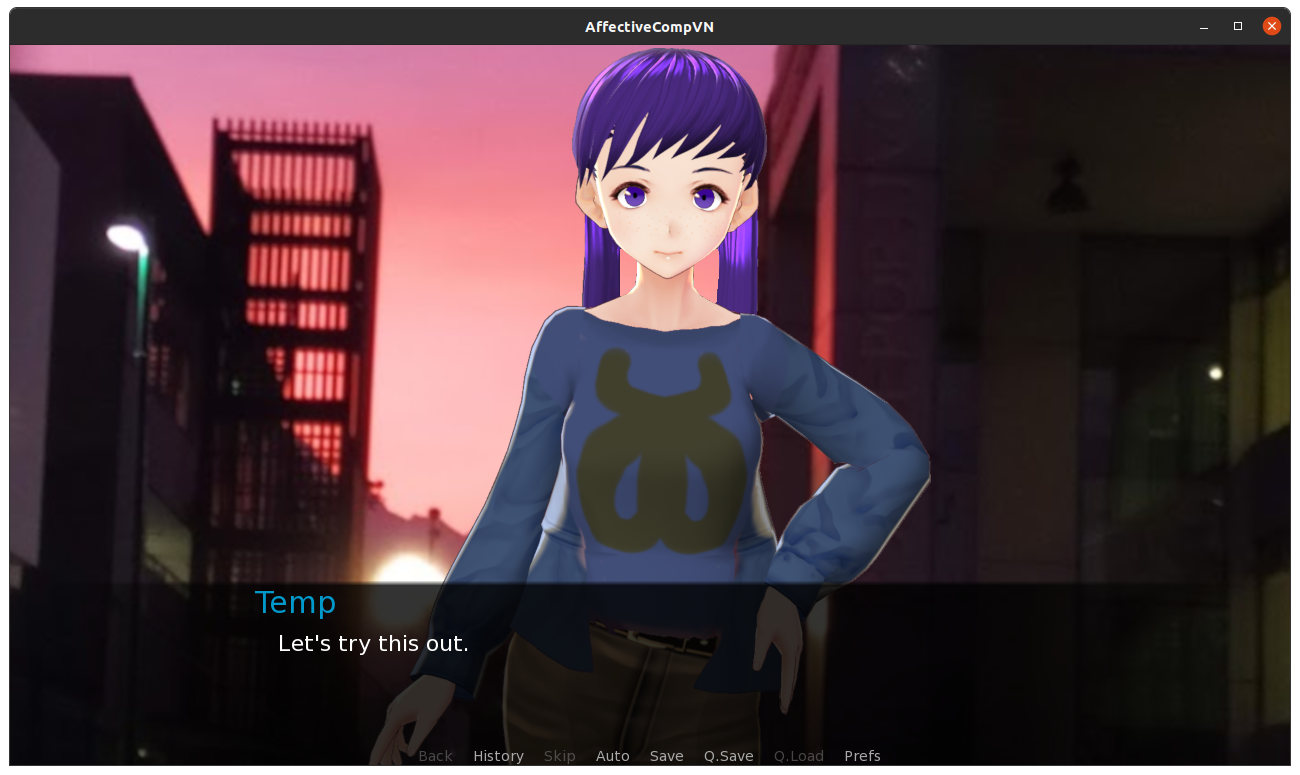
\includegraphics[scale=0.3]{Ren'py}
	\caption{First version of the interface using Ren'py}
	\label{fig:renpy_test_1}
\end{figure}
\begin{figure}[!h]
	\centering
	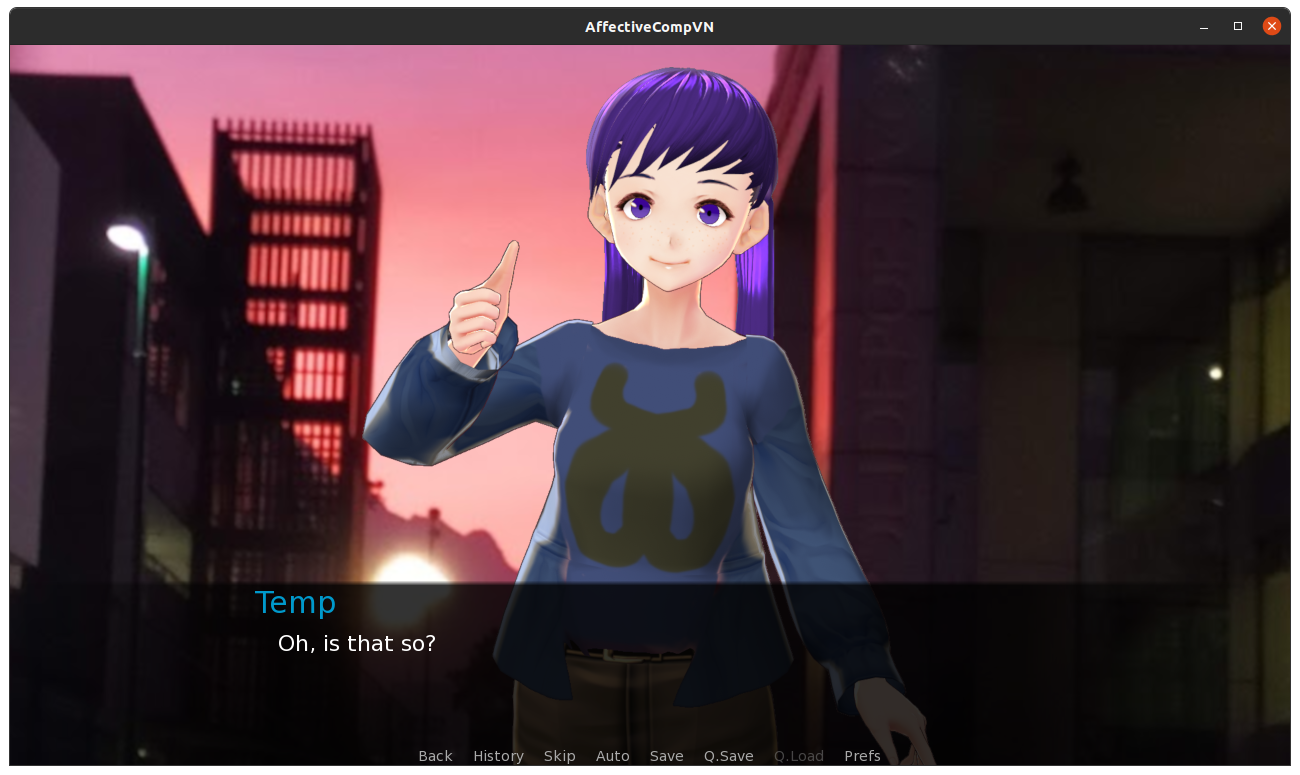
\includegraphics[scale=0.3]{Ren'py_2}
	\caption{Reacting positively to an user's feedback}
	\label{fig:renpy_test_2}
\end{figure}

The current interface is a hybrid between a Pygame screen where the assistant appears to react to the user's input and the console where the user inputs texts to be analyzed.
\pagebreak

\subsection{Assistant}
As for the character that's being used, it's also gone through some changes. Originally the idea was to make a low-poly character render to work with, but since 3D modeling-from-scratch skills exceed the scope of this paper, an alternative software was selected instead. Namely \textit{VRoid}.\\
The main purpose for this assistant is to make the user feel like it's her that they're talking to and not to some faceless machine, while also making it easier to the eyes. A more realistic, less animated style could have been used, but a friendly, less prone to uncanny valley approach to the design was opted for with this in mind.
\begin{figure}[!ht]
	\centering
	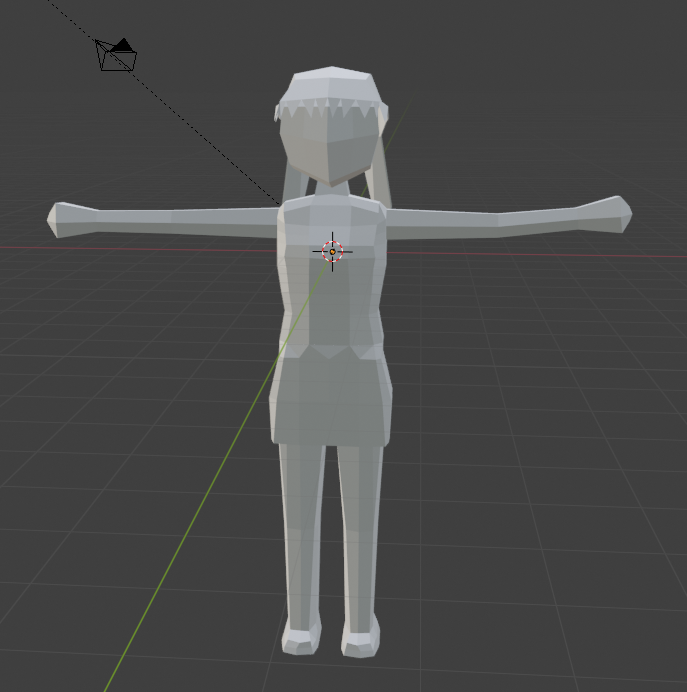
\includegraphics[scale=.5]{Assistant_1}
	\caption{First attempt at 3D modeling an assistant.}
	\label{fig:assistant1}
\end{figure}
\begin{figure}[!ht]
	\centering
	
\includegraphics[scale=.25]{Assistant_2}
	\caption{Assistant Ver. 2, now using VRoid.}
	\label{fig:assistant2}
\end{figure}
\begin{figure}[!ht]
	\centering
	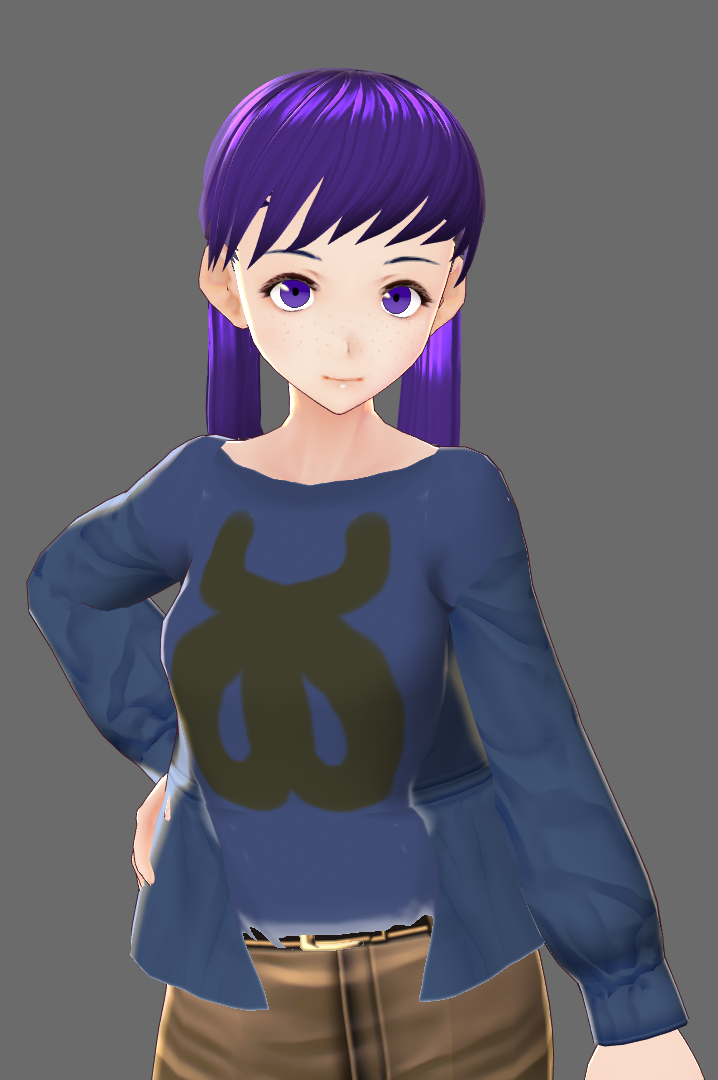
\includegraphics[scale=.25]{Assistant_3}
	\caption{Assistant Ver. 3, the current design.}
	\label{fig:assistant3}
\end{figure}


